\section{Cut-Dependent Analysis}
\label{sec:cutwise}

\subsection{Ranking changes with the cut}

Table~\ref{tab:cutwise} reports engine-mean RMSE at each of the five cuts.
At 0.40, LS-ctx is much better than LTAG on every subset (differences
$-4.170/-1.548/-1.239/-0.904$). At 0.55 the advantage shrinks but remains
negative on all four subsets. At 0.70 the two methods are close. At 0.85 and
0.95 the sign reverses on FD001, FD002, and FD004: LTAG is better than LS-ctx.
The crossover is the source of the apparent conflict between
Tables~\ref{tab:test} and~\ref{tab:validation}. The validation average is
dominated by the early cuts, where the error is large; the test is a single
end-of-life window.

\begin{figure*}[t]
\centering
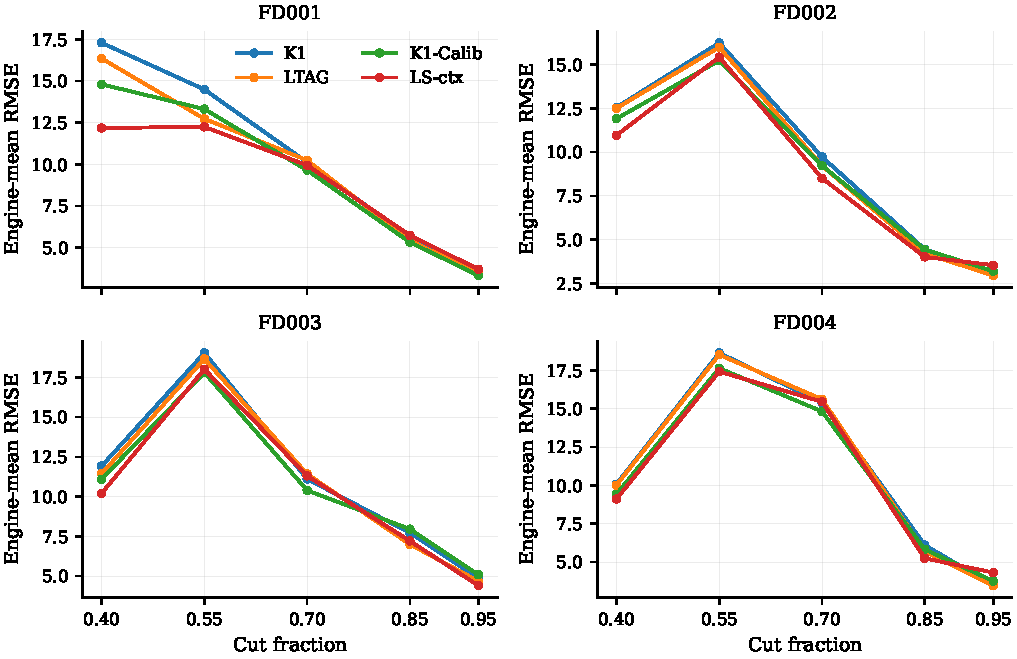
\includegraphics[width=0.95\textwidth]{fig1_cutwise.pdf}
\caption{Cut-wise engine-mean RMSE for K1, LTAG, K1-Calib, and LS-ctx. Calibration
is stronger at early cuts; LTAG is competitive or better near end-of-life.}
\label{fig:cutwise}
\end{figure*}

\begin{table*}[t]
\centering
\caption{Cut-wise validation engine-mean RMSE. LS-ctx is stronger at early cuts;
LTAG is competitive or better at 0.85--0.95. The last column is LS$-$LTAG
(positive = LTAG better).}
\label{tab:cutwise}
\small
\begin{tabular}{llcccccc}
\toprule
Subset & Cut & K1 & LTAG & K1-Calib & LS-ctx & LS$-$LTAG \\
\midrule
FD001 & 0.40 & 17.283 & 16.345 & 14.794 & 12.175 & -4.170 \\
FD001 & 0.55 & 14.485 & 12.724 & 13.308 & 12.243 & -0.481 \\
FD001 & 0.70 & 10.119 & 10.236 & 9.644 & 9.934 & -0.302 \\
FD001 & 0.85 & 5.593 & 5.431 & 5.318 & 5.732 & +0.301 \\
FD001 & 0.95 & 3.473 & 3.437 & 3.322 & 3.705 & +0.267 \\
FD002 & 0.40 & 12.560 & 12.512 & 11.913 & 10.964 & -1.548 \\
FD002 & 0.55 & 16.252 & 15.997 & 15.235 & 15.434 & -0.563 \\
FD002 & 0.70 & 9.731 & 9.218 & 9.229 & 8.510 & -0.708 \\
FD002 & 0.85 & 4.446 & 4.208 & 4.429 & 4.009 & -0.199 \\
FD002 & 0.95 & 3.059 & 2.942 & 3.194 & 3.534 & +0.592 \\
FD003 & 0.40 & 11.922 & 11.440 & 11.093 & 10.200 & -1.239 \\
FD003 & 0.55 & 19.045 & 18.666 & 17.812 & 18.019 & -0.646 \\
FD003 & 0.70 & 11.107 & 11.424 & 10.393 & 11.304 & -0.120 \\
FD003 & 0.85 & 7.722 & 6.994 & 7.952 & 7.207 & +0.213 \\
FD003 & 0.95 & 4.862 & 4.671 & 5.082 & 4.395 & -0.276 \\
FD004 & 0.40 & 10.079 & 10.012 & 9.421 & 9.108 & -0.904 \\
FD004 & 0.55 & 18.644 & 18.523 & 17.643 & 17.426 & -1.097 \\
FD004 & 0.70 & 15.392 & 15.617 & 14.822 & 15.454 & -0.163 \\
FD004 & 0.85 & 6.105 & 5.690 & 5.821 & 5.240 & -0.450 \\
FD004 & 0.95 & 3.468 & 3.459 & 3.752 & 4.310 & +0.851 \\
\bottomrule
\end{tabular}
\end{table*}


\subsection{End-of-life comparison}

At cut 0.95 the best method depends on the subset: K1-Calib is best on FD001
(3.322 vs LTAG 3.437), LTAG is best on FD002 (2.942 vs 3.534 for LS-ctx) and
FD004 (3.459 vs 4.310), and LS-ctx is best on FD003 (4.395 vs 4.671). LTAG is
therefore not uniformly best: it is best on FD002 and FD004, second on FD001 and
FD003, and within 0.28 of the best in every case.

A paired engine bootstrap at 0.95 makes the direction clearer. LTAG is
significantly better than K1-Calib on FD002 ($+0.252$, CI $[0.013,0.495]$) and
FD003 ($+0.411$, CI $[0.078,0.749]$), and significantly better than LS-ctx on
FD002 ($+0.592$, CI $[0.221,0.964]$) and FD004 ($+0.851$, CI $[0.120,1.626]$).
The FD001 difference in favor of K1-Calib ($-0.115$) and the FD003 difference in
favor of LS-ctx ($-0.276$) are not significant. The late-cut evidence supports
LTAG as an end-of-life aggregator, not as a universal one.

\subsection{Per-engine view}

Figure~\ref{fig:winrate} shows the per-engine difference between LS-ctx and
LTAG. LS-ctx wins on 10/20 engines on FD001, 28/52 on FD002, 10/20 on FD003, and
28/50 on FD004. The FD001 median difference is slightly positive (LS-ctx worse),
so the mean gain of LS-ctx comes from a minority of high-error engines. This is
consistent with a tail-calibration interpretation: LS-ctx lowers the largest
errors at the cost of typical accuracy, and its advantage disappears near
end-of-life.

\begin{figure}[t]
\centering
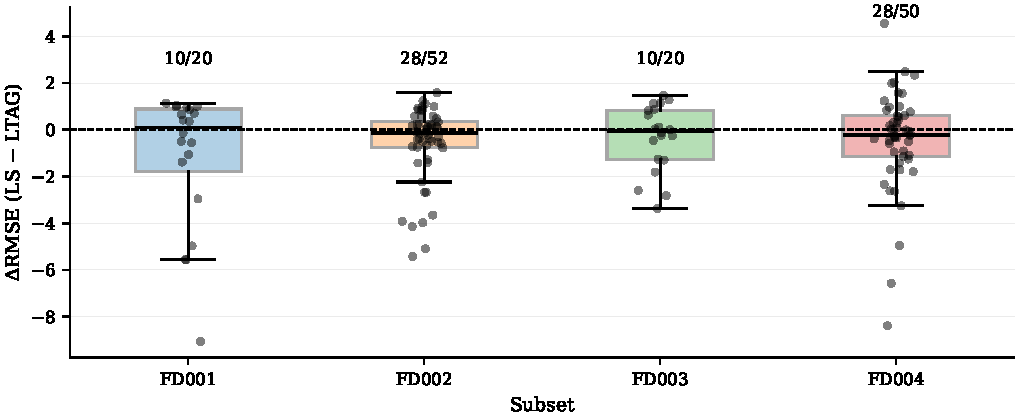
\includegraphics[width=0.48\textwidth]{fig3_winrate.pdf}
\caption{Per-engine $\Delta$RMSE (LS-ctx $-$ LTAG) on validation. Positive means
LTAG is better. LS-ctx wins on 10/20, 28/52, 10/20, and 28/50 engines; the mean
gain is driven by a minority of high-error engines.}
\label{fig:winrate}
\end{figure}

\subsection{What this means for evaluation}

A validation average over cuts is not a proxy for the end-of-life test. The same
two methods can rank in opposite orders depending on the cut composition. We
therefore recommend that multi-window RUL papers report a cut-wise table (or at
least the 0.95 cut) alongside the average. The protocol in this paper is a
minimal version of that recommendation: five cuts, engine-mean and pooled RMSE
separately, and an explicit end-of-life column.
